\chapter{Results}
 In the previous chapter, a simple feedforward network with two layers was devised. The responses of various convergent connections in the network to static and oscillating input are discussed in this section. The goal of this study is to investigate how information transfers as inferred from the output firing rate can be modulated by the level of synchronization of the input and which convergent connection rule has the highest output response with regard to this input synchronization.

First, we describe a unique activity map under various types of input and various types of convergent connections rules. We then show an increase in the output firing rate when the feedforward connection strength increases and when the synchronization level during the input increases. We demonstrate that the Uniform-Uniform convergent rule (UU) has the highest response gain from a static input to an oscillating input when compared to other convergent rules. Finally, we reveal that the UU rule has the highest induced spike gain and that it is highly dependent on the phase of the input oscillation. An explanation of why the UU rule is most sensitive to synchronized input based on the idea of temporal summation was also given.

%
%
%%Response Function
%
%Figure 1. Network of different types of convergence 
%
%Figure 2. Firing rate increases for oscillating input
%
%Figure 3. Gain function of firing rate for oscillation is greatest in UU
%
%Figure 4. Gain function of induced post-synaptic spike for one pre-synaptic spike is highest in UU model
%
%Figure 5. Post-synaptic activity is most tuned for oscillation in UU model
%


% Add this Question and Hypothesis in the method part too
\section{The activity map of the target layer shows the unique response of each convergent rule and input pattern combination}
 For each input pattern and convergent rule combinations, an activity matrix is formulated by assigning each element as the average firing rate of the target layer under the given convergent conditions ( $r_i$, $w_i$). Three convergent rules and three input levels are multiplied to make nine cases of an activity matrix, as shown in figure ~\ref{fig:ActivityMatrix} 
A contour plot from this matrix serves to construct an activity map for each condition (Figure~\ref{fig:ActivityMap}). In the activity map, a lighter color means a higher firing rate.  In all cases, when convergent conditions increase, the response increases. However, the rates of increase differ in each case, as can be easily observed when comparing the same position of the map in all cases (red dot position; $r_i$ = 80, $w_i$ = 80 ). 


%Activity Matrix
\begin{figure}[!h]
	\centering
	\includegraphics[width=0.9\textwidth]{figures/Result_ActMatrix}
	\caption{The activity matrix shows the response of a feedforward network under different conditions. Row~: Convergent Rules; Gaussian-Gaussian(GG), Uniform-Uniform(UU), and Uniform-Exponential(UE) , Column ~: Input pattern; static, weak oscillation, and strong oscillation input.}
	\label{fig:ActivityMatrix}
\end{figure}

%Activity Map
\begin{figure}[!h]
	\centering
	\includegraphics[width=0.9\textwidth]{figures/Result_ActMap}
	\caption{Activity Map created from a contour plot of the activity matrix. Red dots show the locations of identical convergent conditions in each case, but they have different responses due to the input pattern and convergent rules used.}
	\label{fig:ActivityMap}
\end{figure}


 To explore the role of each convergent condition parameter, the output firing rates were plot when one parameter is fixed. If range of the connection is fixed, the output  firing rate versus the weighting factor parameter is plotted (Figure~\ref{fig:ObservedRfix}). Likewise, if the weight condition is fixed, the output  firing rate versus the range  parameter is plotted (Figure~\ref{fig:ObservedWfix}). 
When observing the changes in the output firing rate, we found that a strong oscillating input has the highest response compared to the other input patterns in all cases.  


%Fix R , and fix W 
\begin{figure}[!h]
	\centering
	\includegraphics[width=1\textwidth]{figures/Result_fixRange}
	\caption{The observed responses of the network when the range of connections is fixed and when the weight varies}
	\label{fig:ObservedRfix}
\end{figure}

\begin{figure}[!h]
	\centering
	\includegraphics[width=1\textwidth]{figures/Result_fixWeight}
	\caption{The observed response of the network when the strength of the connection (or weight) is fixed and when the range of connections varies}
	\label{fig:ObservedWfix}
\end{figure}


\section{A feedforward network with strong oscillation input has the highest output firing rate}
% The response function, average output firing rate over total feedforward 
 According to the observation in the previous part, an oscillating input gave a higher response compared to a static input. Next, a general analysis is conducted with all the convergent conditions by examining the relationship between the output firing rate and the total feedforward strength ( or the summation of the total weight, as introduced earlier).  From this plot (Figure ~\ref{fig:ResFun} ), it can clearly be seen that as the total feedforward connection strengthens, the output firing rate also increases.
 In addition, the firing rate with all convergent rules increases for an oscillating input compared to a static input case. The slope of this plot can be considered as the gain or average firing rate per unit of feedforward strength.  Higher gain values mean that the feedforward network can transfer more spikes to the output layer with the same connection strength used with the lower gain values. The slopes or gains from this response function are plotted in Figure~\ref{fig:ResFunDiff}. This plot clearly shows for all convergent rules, a strong oscillation  input has the highest gain compared to the weak oscillation and static inputs.  If we examine this further by examining the differences in the slopes of the strong oscillation input and the static input according to all convergent rules, we find that the Uniform-Uniform model has the greatest differences in the gain values, as shown in Figure~\ref{fig:ResFunDiff} B. 


\begin{figure}[!h]
	\centering
	\includegraphics[width=1\textwidth]{figures/Result_MeanFr_sumW}
	\caption{The response function (mean firing rate vs. total feedforward strength) of UU, GG, and UE from left to right. The firing rate increases when the connection strengthens.}
	\label{fig:ResFun}
\end{figure}


\begin{figure}[!h]
	\centering
	\includegraphics[width=1\textwidth]{figures/Result_MeanFr_sumW_slope}
	\caption{Comparison of the slope or gain. A. The firing rate increases for an oscillating input. B. The UU model has the highest difference in the firing rate between a strong oscillation and a static input.}
	\label{fig:ResFunDiff}
\end{figure}



\section{The Uniform-Uniform model has the highest response gains from a static input to an oscillating input}
 In the previous section, the Uniform-Uniform model showed the highest oscillation-static differences in the gain (average output firing rate over the total feedforward connection strength). In addition, the previous results showed that the feedforward network with an oscillating input has a higher response in the target layer than the static input case.  
Next, in order to explore how much the response from an oscillating input increases from a static input, the firing rate of each condition was scattered onto the static input axis and the oscillating input axis (Figure~\ref{fig:ResFunDiffOscS}). A linear fitting was established for data from each of the convergent rules, i.e., the Gaussian-Gaussian(GG),Uniform-Uniform(UU), and Uniform-Exponential(UE) rules. The slope of each convergent rules population is then determined and compared. The slope of this fitted line is defined as the gain (output firing rates with an oscillating input over those when static inputs were given). These results are plotted in Figure ~\ref{fig:ResFunDiffOscS_hp}. Because there are two types of oscillation inputs, two comparisons can be made: weak oscillation versus static(WO-S), and strong oscillation versus static(SO-S). We found that in both comparisons of WO-S and SO-S, the Uniform-Uniform rule has highest gain from static to oscillation compared to the other convergent rules. The gain can infer the sensitivity of each feedforward network to the synchronization level of input. 



\begin{figure}[!h]
	\centering
	\includegraphics[width=1\textwidth]{figures/Result_OscFR_StaticFR_Scatter}
	\caption{Comparison of the output firing rate of a static input and an oscillating input. WO-S and SO-S are compared between a static input with weak oscillation and strong oscillation respectively.}
	\label{fig:ResFunDiffOscS}
\end{figure}


\begin{figure}[!h]
	\centering
	\includegraphics[width=0.5\textwidth]{figures/Result_OscFR_StaticFR_bar}
	\caption{The Uniform-Uniform model had the greatest gain from static to oscillation inputs.}
	\label{fig:ResFunDiffOscS_hp}
\end{figure}

\section{The Uniform-Uniform model has the highest number of induced spike gains on the target layer from one spike in the source layer}
 From the previous result, the UU model  has highest response gain from a static input to an oscillating input. An additional analysis was conducted to quantify the number of output spikes that one input spike can create. This analysis started by counting the number of postsynaptic spikes in the target layer following each presynaptic spike in the source layer when there is a connection between the layers. Then, this count was normalized with the total number of spikes to create an induced spike plot. The area under the first peak of the curve cut by the baseline activity is the yield-induced spike.  By scattering these induced spikes of static and oscillating inputs, we can investigate the relationship between the levels of synchronization in the input. The gain function can then be calculated from the ratio between the induced spike from an oscillation input and the induced spike from a static input(Figure ~\ref{fig:InduceCurve}. ). The average gain of each convergent rule is shown in Figure~\ref{fig:InduceBar}  with two oscillation-static comparisons. The results show that the number  of induced spikes in the Uniform-Uniform model is highest compared to the other two cases ( GG was second, while UE had the lowest gain). In addition, the overall gains of the induced spikes in the SO-S case are higher than in the WO-S case, which can be expected as the synchronization level in the WO is less than in the SO input. The highest gain in the induced numbers of spikes shows that the Uniform-Uniform convergent rules can produce more spikes per input spike. This result represents an analysis at the cell level compared to the previous analysis, which examined these properties at the network level. 



\begin{figure}[!h]
	\centering
	\includegraphics[width=1\textwidth]{figures/Result_Induced_curve}
	\caption{Example plots of the timing of an induced target spike from a spike in the source layer. The shaded area, the area under the first peak  to the baseline level, represents the number of total induced spikes.}
	\label{fig:InduceCurve}
\end{figure}

\begin{figure}[!h]
	\centering
	\includegraphics[width=0.4\textwidth]{figures/Result_Induced_bar}
	\caption{The number of induced spike gains from a static to an oscillation input. UU has the highest gain with both levels of oscillation. (T-test, $p < 0.05$)} % t-test.
	\label{fig:InduceBar}
\end{figure}

 
\section{The output spikes in target layer of the Uniform-Uniform model depend mostly on the phase-lock to oscillation}
  All previous results showed that the strong oscillation input leads to the highest response compared to weak oscillation and static inputs. Also, the Uniform-Uniform convergent rule has the highest sensitivity to a change from a static input to an oscillating input. 
The next question is how output spikes are related to the phase of the input pattern and how convergent rules behave differently given this type of phase tuning. 
The output response-input phase relationship is determined by the count output spike timing during one period of input oscillation and by then summing up all of the periods available in a simulation.  The result is shown in Figure~\ref{fig:PhaseCurve}. It appears that the responses are phase-locked to the crest of the oscillating input.
Because we are interested in the gain or differences in these values with an oscillating input over a static input, the plots for each of the convergent rules are normalized by the relevant spike number in static input. From this curve, the full width half maximum (FWHM) values were measured and the average values then plotted in a bar graph (Figure~\ref{fig:PhaseBar}). A small width means that the responses are sharply tuned to the phase of the oscillated input pattern. For a comparison between the strong oscillation and static input, the UE showed the widest width, while UU and GG rules showed small widths. Comparing the UU and GG models, they are shown to be significantly different with smaller widths for the UU rule. The WO-S comparison showed a similar result but overall a wider width in all cases. Therefore, this evidence suggests that the Uniform-Uniform model is mostly tuned to the phase of the input oscillation.




\begin{figure}[!h]
	\centering
	\includegraphics[width=1\textwidth]{figures/Result_PhaseTune_curve}
	\caption{Spiking timing in one period of an oscillation input pattern. Left, an example of a tuning plot . Right, the spiking timing normalized by that of a static input, the width measurement, and the full width at half maximum (FWHM).} 			\label{fig:PhaseCurve}
\end{figure}

\begin{figure}[!h]
	\centering
	\includegraphics[width=0.5\textwidth]{figures/Result_PhaseTune_bar}
	\caption{The UU convergent rule has the smallest width indicating the highest tuning to an oscillation input compared to the GG and UE rules} 
	\label{fig:PhaseBar}
\end{figure}


\section{The Uniform-Uniform model has highest sensitivity to synchronized input because of its optimal distribution of weighting factor}
 The Uniform-Uniform convergent rule shows the highest sensitivity to the level of synchronization in the input pattern, as shown by the response gain from a static to an oscillating input, by the number of induced spike gains, and by the phase-locked condition to the oscillation.  The next question must explain what occur during the Uniform-Uniform convergent rules  that make it sensitive to changes in the synchronization level of the input.

\begin{figure}[!h]
	\centering
	\includegraphics[width=1\textwidth]{figures/WeightDistForOneCell}
	\caption{The distribution of the weighting factors of convergent connections to a target cell} 
	\label{fig:WdistOne}
\end{figure}

 We confirmed that the distribution of the connection probability and the connection strength are as we designed them in the methodology chapter (Figure~\ref{fig:WdistOne}). Moreover, the distributions of the weighting factors of all cells in the target layer were different from that of a single target cell due to the stochasticity in the system, as shown in Figure ~\ref{fig:WdistNN}). According to this distribution, the UE model has an exponential distribution, as expected. The UU model has a normal distribution due to stochastic environment. The Gaussian-Gaussian model has a nearly flat distribution. The Gaussian distribution has a high weighting factor in the center population and has a lower weight value at the boundary. However, due to the increase in stochastic area covered by the filter at the boundary, where stochastic connection probability and weighting factor are low, compensation for the low connectivity effect occurred thus raising the low weight. As a result, the GG model has a flat distribution (Figure~\ref{fig:WdistNN}).  When comparing the cumulative sums of these distributions, the UU model clearly has a narrow range of strength compared to a conventional model such as GG model.

\begin{figure}[!h]
	\centering
	\includegraphics[width=1\textwidth]{figures/WeightDistForNetwork}
	\caption{The distribution of the weighting factors of all convergent connections to the target layer. Small figure - Top: cumulative distribution function of the weight distribution for all types. Bottom: A plot of a 2D Gaussian filter showing an increase in the ring area at boundary where the Gaussian value is low compared to the inner area, which has a high Gaussian value but it limited space.} 
	\label{fig:WdistNN}
\end{figure}


\begin{figure}[!h]
	\centering
	\includegraphics[width=1\textwidth]{figures/WeightDistForSchematic}
	\caption{A schematic figure using the idea of temporal summation \cite{magee1999dendritic}  to explain why the UU model has the highest sensitivity to the level of synchronization during an input} 
	\label{fig:WdistSchematic}
\end{figure}



 The distribution of the weighting factor or strength of a feedforward connection is a key to explain its sensitivity to the synchronization level of the input.  We divided the group of weighting factor into three groups according to their range, low, middle, and high, and then use this to explain the feedforward connection characteristics and its responses. At a high connection strength, a spike from the source cell can create a spike in the target layer. At a low connection strength level, it is difficult to create a spike cell with only a single spike from source layer. However, the middle range of the connection strength is the range in which the probability of creating a spike is not certain but depends on the pattern of the input spikes; this can be explained by considering the idea of temporal summation during cell conductance (Figure~\ref{fig:WdistSchematic}). When there is no oscillation in the input, the spikes arrive at the postsynaptic cell individually (not overlapping or too close to each other).  In this middle range of connection strength, the conductance of these single spikes cannot reach the threshold of action potential and therefore cannot produce a spike in the target cell.  If oscillating inputs are given at this same middle range of the connection strength, however, there would be many spikes with short inter-spike intervals and many overlapping spikes (because they are synchronized), which then increase the conductance sum, as in temporal summation concept, causing a spike in target cell. The connection strength in the UU model clustered around the middle range is why the changes during the static and the strong oscillation inputs in the UU model are the highest. 




%
%\section{Prof's suggestion}
%General Note : If you fix trial number to some n value --> explain why it is enough.  
%What are the meaning of these result in biological system
%\subsection{Proved your hypothesis}
%\paragraph{Hypothesis}  The brain (is it too big or too general?) need interlayer communication that optimized cost of the connection 
%which is achieved by the synchronized neural activity on source layer and statistical wiring diagram( with Gaussian distribution of connectivity and connection strength)
%
%\paragraph{Proving the Hypothesis}  Compare differences in these three cases of connection (Gaussian, uniformly random, random with negative exponential) of input variations
% ( osc  vs. no osc  ; varies F and Amp ) 
% The measurement can be  1) Fr ,  2) Spike Correlation, 3) Spike Pattern (Ex. M1 activity according to Input oscillating pattern, how is the phase affect the result etc )
%

%\begin{center}
%....................
%OLD
%....................
%\end{center}
%\section{ Answer to RQ1 : The computer simulation resemble experimental results of animal study}
%
%\subsection{ The single cell properties of computational model and the whole cell patch clamp recording shows the same behavior}
%
%Figure .1.1: Comparing the sample membrane potential trace of WT and KO during hyperpolarize current injection and depolarize current injection
%
%Figure .1.2: Comparing the number of bursting spikes and tonic spikes between the simulated cell and experimental data
%
%
%\subsection{  The cell population properties of computational model and the MUA cells recording shows the same behavior}
%
%Figure .1.3 : Comparison of mean and standard deviation of observed firing rate in cell population in computational model and experimental data
%
%
%\subsection{ Neuron activities during light-off period (no photoactivation)}
%
%Figure .1.4 The baseline activities of neural population during light-off period show no significant different between WT and KO
%
%
%\subsection{ Neuron activities during photoactivation}
%
%Figure .1.5 The delay and peak of rebound spiking activity of WT and KO are significantly different. The WT shows short rebounding period and higher peak of neural activities
%
%
%\subsection{ The coherence between VL and M1 layer shows that correlated neural activities after photoactivation ( the rebound bursting spikes) drives activity in M1}
%
%Figure~\ref{fig:sample} The coherence between VL’s MUA and M1’s LFP
%
%\begin{figure}
%	\centering
%	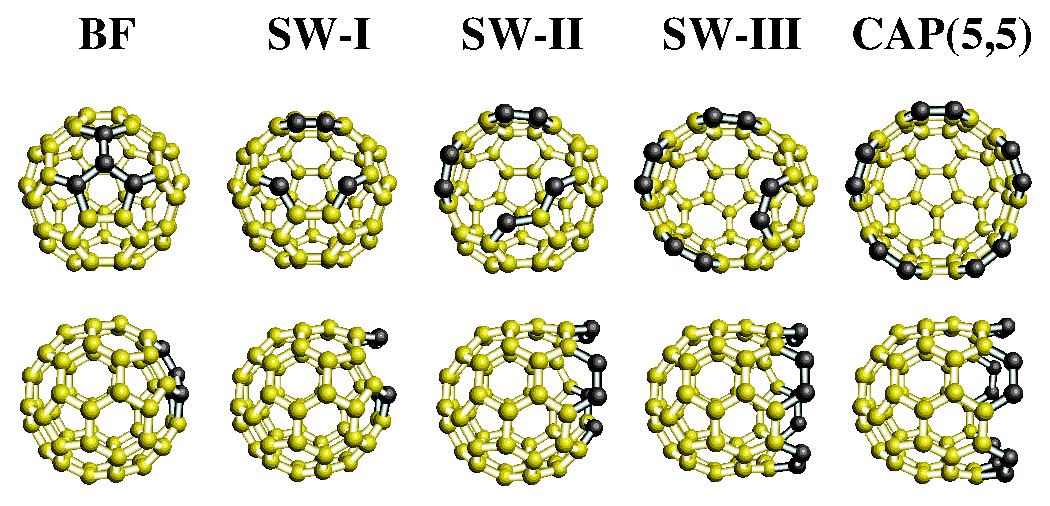
\includegraphics[width=0.5\textwidth]{figures/sample-fig1}
%	\label{fig:sample}
%	\caption{Sample Figure}
%\end{figure}
%
%\section{Answer to RQ2 : Computational simulation predicts causal relationship of exceed motor command in M1 from VL in Parkinson’s disease patient}
%
%\subsection{ The high synchronization (correlated neural activities) in VL but not average firing rate can drive M1’s motor command}
%
%
%Figure .2.1 The high synchronized neural activities during bursting can drive M1 in WT types but not KO, even though the average firing rate if WT and KO are not significantly difference
%
%
%\subsection{  The high synchronization level can be achieved by bursting. The demolishing of bursting in WT neurons result in the absent of synchronization in neuron population}
%
%Figure .2.2 Schematic diagram of how the bursting activity cause high synchronization in neuron population
%
%\subsection{ The Analysis of information transfer from VL to M1 : The information in VL can transfer to M1 when the neuron population in VL are synchronized }
%
%Figure .2.3 the neural information from VL is transferring to M1 only when the neural activities in VL are synchronized.
%
%Figure .2.4 the level of information transfer between VL and M1 is proportionally to the synchronization level in VL
%
%\subsection{ Artificially generated bursting in KO neurons result in high synchronization level of neuron population which can drive M1’s motor command
%}
%Figure .2.5 successfully generated bursting behavior in KO with similar bursting behavior generated by T-Type Calcium channel in WT
%
%Figure .2.6 The artificial bursting behavior in KO result in high level synchronization level of neural population and this high synchronized neural 
%population can drive M1
%
%\subsection{ Artificially activated VL neural population in theta and beta frequencies result in motor command from M1with the same frequency band with what observed in Parkinson’s disease patient.}
%
